\documentclass[10pt]{report}

\usepackage{talks}
\newcommand{\expect}[1]{\mathbb{E}\!\left[ #1 \right]}
\newcommand{\reals}{\mathbb{R}}
\usepackage{mathpazo}
\usepackage{sourcecodepro}
\usepackage{tikz}
  \usetikzlibrary{arrows.meta, angles, quotes, calc, positioning, shapes}
\renewcommand{\baselinestretch}{1.05}
\newcommand{\ddfrac}[2]{\frac{\strut \displaystyle #1}{\strut \displaystyle #2}}
\newcommand{\pos}[2]{#1^{(#2)}}
\newcommand{\drw}[2]{#1_{#2}}
    
\begin{document}

\sf
\mbox{ } \\
\spc{\LARGE\bfseries \color{MidnightBlue}{Scaling Bayesian Inference:}}
\\[4pt]
\spc{\Large\bfseries \color{MidnightBlue}{Up, out, and to GPUs}}
\vfill
\noindent 
\spc{\large\bfseries \color{MidnightBlue}{Bob Carpenter}}
\\[8pt]
\spc{\small Center for Computational Mathematics}
\\[-1pt]
\spc{\small Flatiron Institute}
\\[2pt]
\spc{\footnotesize \url{bcarpenter@flatironinstitute.org}}
\noindent
\\
\vfill
\noindent\spc{\footnotesize 2026 SIAM: Parallel Processing for Scientific Computing}
\hfill

\includegraphics[width=1.25in]{img/flatiron-logo.png}


\sld{The constraints of current compute scaling}
\begin{itemize}
\item \myemph{Single CPU growth} used to drive scientific computing:
  \begin{subitemize}
  \item speed and memory doubled every 18 months (!)
  \end{subitemize}
\item Modern compute grows by \myemph{multi-tasking}.
  \begin{subitemize}
    \item Processors (esp.\ GPU) are \myemph{slower} and more
      \myemph{memory bound}.
    \item \myemph{CPU scaling} modest but flexible ($10^2$ vs. $10^4$
      processors)
    \item Mac \myemph{integrated memory} is a game changer
    \item GPU scaling requires blockwise-SIMD algorithms for performance
    \end{subitemize}
    \vfill
\item \footnotesize \myemph{global RAM shortage} from underestimating
  need
  \begin{subitemize}
    \footnotesize
  \item prices up 5x or more; supply chain iffy
  \item should resolve in 18 months or when AI bubble bursts
  \end{subitemize}
\end{itemize}

\sld{Problem: Bayesian inference via Monte Carlo}

\begin{itemize}
\item Given:
  \begin{subitemize}
  \item known/observed data $y$,
  \item unknown/latent parameters $\theta$, and
  \item a target posterior density $p(\theta \mid y)$ \ {\footnotesize (known up to a constant)}
  \end{subitemize}
\item Draw a posterior sample $\drw{\theta}{1},\ldots,\drw{\theta}{M}
  \sim p(\theta \mid y)$
\item Plug in for posterior inference; e.g., estimate expectations
  $$\mathbb{E}[f(\theta) \mid y] \approx \frac{1}{M} \sum_{m=1}^M f(\drw{\theta}{M}).$$
\end{itemize}

\sld{Fools gold standard: Markov chain Monte Carlo}
\begin{itemize}
\item $\drw{\theta}{1}, \ldots, \drw{\theta}{m}, \ldots$ is a
 \myemph{Markov chain} with target stationary distribution
\item Markov chains intrinsically \myemph{sequential} with ``random'' transitions
  $$\drw{\theta}{n + 1} = g(\drw{\theta}{n})$$
\item Transitions \myemph{deterministic} w.\ fixed
  pseudo-random number generator.
\vfill
\item \myemph{Slow} and \myemph{not very scalable}
  \begin{subitemize}
  \item even when it works (i.e., mixes well enough)
  \end{subitemize}
  \vfill
\end{itemize}

\sld{Current tMCMC approaches bottlenecked}
\begin{itemize}
\item \myemph{Parallel proposals} seem reasonable
  \begin{subitemize}
    \item Only logarithmic speedup in processors
  \end{subitemize}
\item \myemph{Parallel Markov chains} multiple effective sample size
  \begin{subitemize}
  \item Bottleneck: sequential burn-in
  \end{subitemize}
\item \myemph{Sequential Monte Carlo} evaluates many particles in parallel
  \begin{subitemize}
  \item Bottleneck: sequential ``annealing'' algorithm (it's in the name)
  \end{subitemize}
\item \myemph{Ensemble Monte Carlo} methods for auto global curvature adaptation
  \begin{subitemize}
  \item Bottleneck: only at stationarity, sequential to get there
  \item Hope is that parallelism improves adaptation
  \end{subitemize}
\end{itemize}

\sld{Current variational approaches}
\begin{itemize}
\item Most variational inference leads to a very poor approximation.
\item \myemph{Stein variational inference} optimizes location of multiple
  particles to minimize Wasserstein distance to target.
  \begin{subitemize}
    \item Should have near-optimal fit if Wasserstein approximation is good
    \item Bottleneck: sequential, stiff optimization problem
    \end{subitemize}
\item \myemph{Normalizing flows} and \myemph{diffusions}
  \begin{subitemize}
    \item Efficient parallelization of neural network layers makes
      possible.
    \item Can fit target densities that frustrate MCMC.
    \item Bottlenecks: sequential transform, feedfroward neural network layers
  \end{subitemize}
\end{itemize}

\sld{Lock-free, parallel convergence monitoring}
\begin{itemize}
  \item \myemph{$\widehat{R}$ statistic} converges to 1 for chains with same
    stationary distribution
  \item \myemph{One chain per thread} accumulating mean and variance
    using Welford
  \item \myemph{Monitor thread} reads mean/variance/count from
    latest-only single-writer/single-reader queue.
  \item Monitor computes $\widehat{R}$ and terminates if below
    threshold.
  \item Do not need latest, so \myemph{synchronize with lock-free atomics}
    \begin{subitemize}
      \item mean/variance/count in single precision is 12 bytes
      \end{subitemize}
    \item Only monitor log density parameter as it is usually slowest.
\end{itemize}

\sld{A bit harder for adaptation monitoring}
\begin{itemize}
\item We're adaptating a \myemph{step size} (scalar) and a \myemph{diagonal mass matrix}
  (vector).
\item Use a \myemph{triple buffer} for our single-writer/single-reader
  queue.
\item \myemph{Step size convergence} if each chain's step size is
  within tolerance of the geometric average across chains.
\item \myemph{Mass matrix convergence} if each chain's standardized L2
  norm is within tolerance of the geometric average across chains.
  \vfill
\item GitHub: \texttt{flatironinstitute/walnuts}
\item \myemph{Nearly no overhead} on my Mac Studio.
\end{itemize}

\sld{Parallelizing MCMC across the sequence length}
\begin{itemize}
\item Major breakthrough could \myemph{save MCMC} from obsolence
\item David M. Zoltowski, Skyler Wu, Xavier Gonzalez, Leo
  Kozachkov, Scott W. Linderman. 2025.  \myemph{Parallelizing MCMC across the sequence
    length}. {\slshape NeurIPS}.
\vfill
\item 
  Evaluates \myemph{length-$M$ chains} with \myemph{$M/2$ processors} in
  \begin{center}
    \myemph{---$\mathcal{O}(\log M)$ time---}.
    \end{center}
\item Given initial state and RNG, Markov chain is
  \begin{center}
    \myemph{---recovered to machine precision---}.
    \end{center}
\end{itemize}

\sld{Generating a Markov chain by optimization}
\begin{itemize}
\item Given an \myemph{initialization} $\drw{\theta}{0}$ and \myemph{PRNG}
\item Let $g_m(\cdot)$ be the deterministic transition function at step $m$
\item \myemph{Residual vector} fo a state $\drw{\theta}{1}, \ldots,
  \drw{\theta}{M}$ is the sequence of transition discrepancies
  $$
  \textrm{res}(\theta)
  = [\drw{\theta}{1} - g_1(\drw{\theta}{0}), \ \
     \drw{\theta}{2} - g_3(\drw{\theta}{1}), \ \
     \ldots, \ \
     \drw{\theta}{M} - g_M(\drw{\theta}{M-1}].
     $$
   \item \myemph{Loss} is the squared $L_2$ norm of the residual,
     $$
     \textrm{loss}(\theta)
     = ||\textrm{res}(\theta)||_2^2
     = \textrm{res}(\theta)^\top \cdot \textrm{res}(\theta).
     $$
\item \myemph{Zero loss} only for target chain (otherwise positive)
\end{itemize}

\sld{The algorithm}
\begin{itemize}
\item[] $\theta^{(n)}_m$ is step $m$ of chain for the $n$-th algorithm
  iteration.
\end{itemize}
\vfill
\begin{enumerate}
\item Set $\drw{\theta}{m}^{(0)} = \drw{\theta}{0}$ for all $m$
\item for $n \in \{ 1, 2, \ldots \}$:
  \begin{enumerate}
  \item $\theta^{(n)} = \textrm{quasiNewtonStep}(\theta^{(n-1)})$
  \item if $\textrm{loss}(\theta^{(n)}) < \tau$:
    \begin{enumerate}
    \item return $\theta^{(n)}$
      \end{enumerate}
    \end{enumerate}
\end{enumerate}
\vfill
\begin{itemize}
\item Rest is important detail about evaluating the quasi-Newton step.
\end{itemize}

\sld{Length 100K Markov chain in 147 iterations}
\begin{itemize}
\item Parallel HMC, Rosenbrock density, quasi-Newton, \myemph{gray target}
  \\
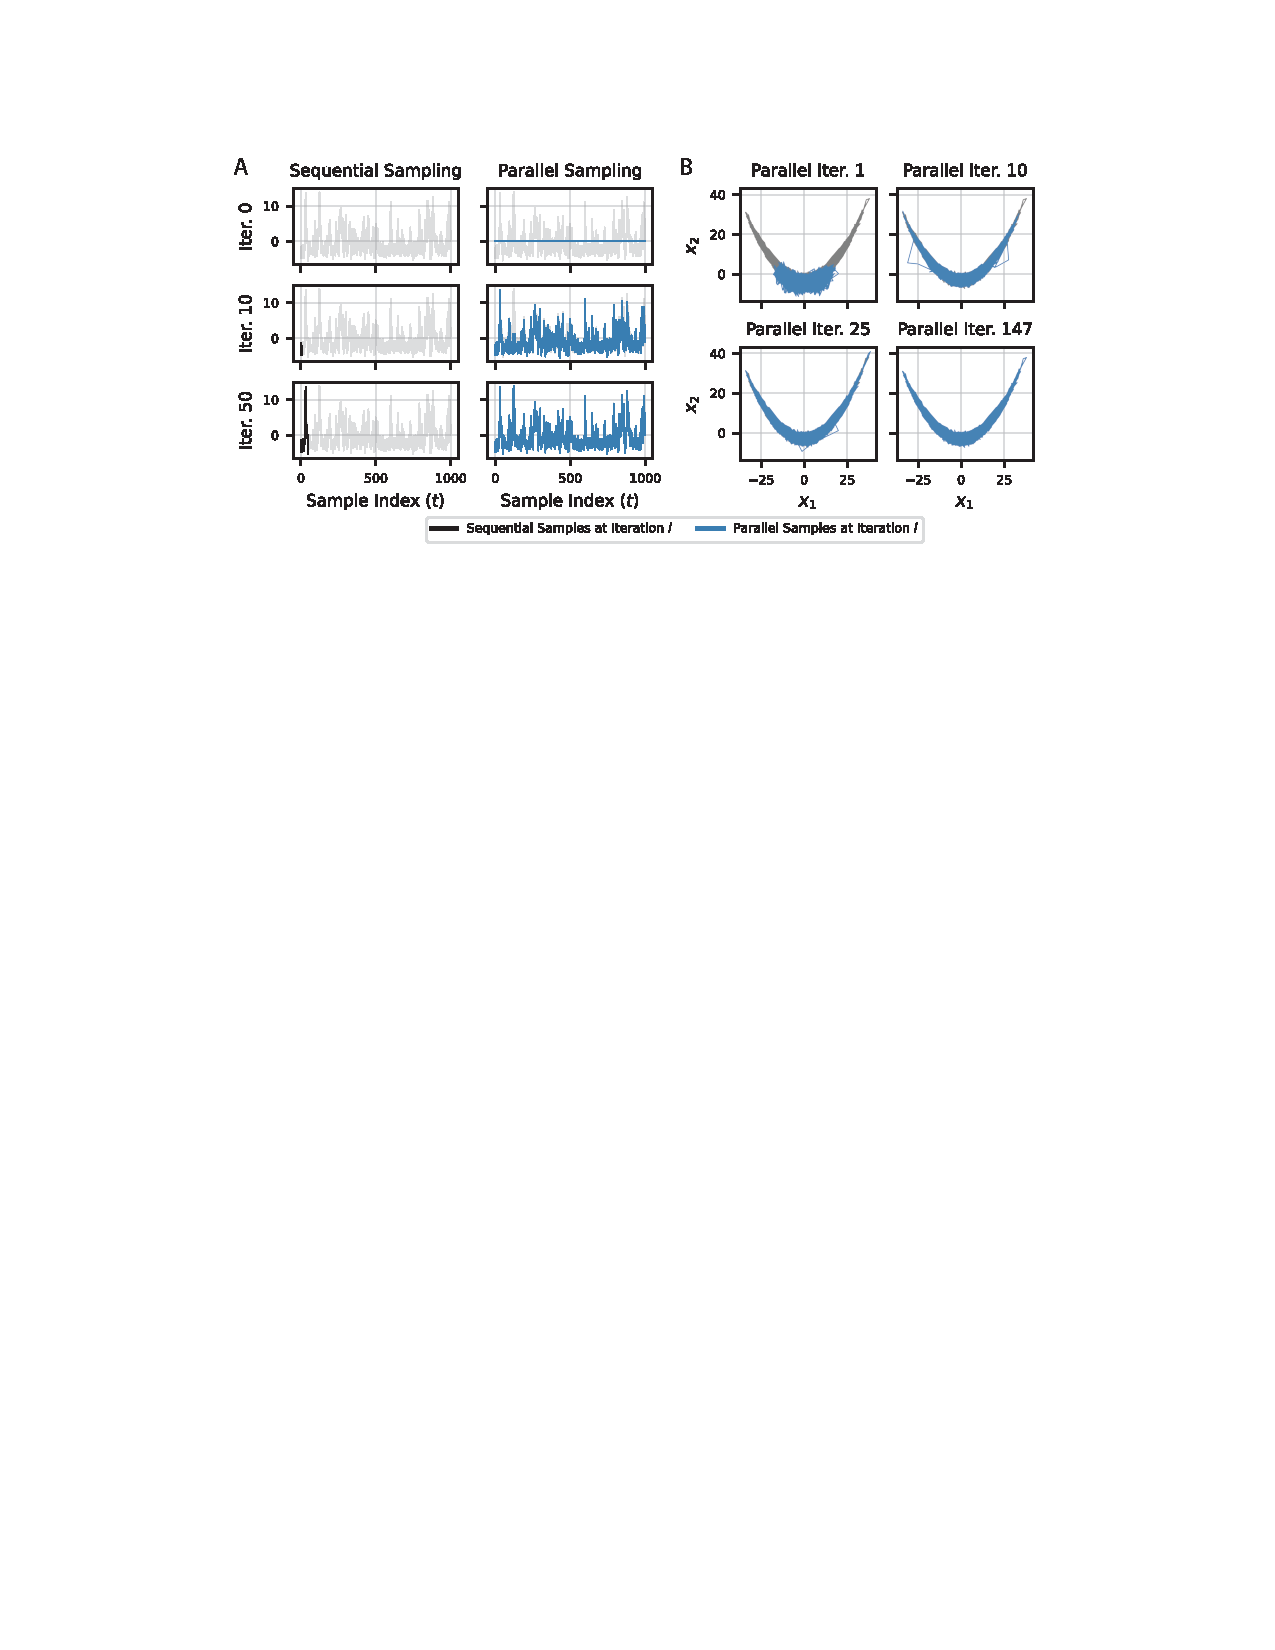
\includegraphics[width=0.8\textwidth]{img/opt-mcmc.pdf}
\end{itemize}

\sld{It's a really high-dimensional optimization}
\begin{itemize}
\item For unadjusted MCMC, the update function $g_m(\theta)$ is
  \myemph{differentiable}
\item For unbiased MCMC, need \myemph{continuous relaxation of accept/reject}.
\item For scalability, need \myemph{quasi-Newton}
  \begin{subitemize}
  \item Zoltowski et al.\ use \myemph{Jacobian's block structure}
    for block-diagonal quasi-Newton
  \end{subitemize}
\item Quasi-Newton \myemph{requires second-order derivatives} of
  target log density
\end{itemize}

\sld{Quasi-Newton update is sequence evaluation}
\begin{itemize}
\item Quasi-Newton update \myemph{requires a scan} (i.e., prefix sum)
\item Scan operations are \myemph{Jacobian-based approximations} of transitions.
\item \myemph{Parallel prefix-sum algorithms} scan in
  $\mathcal{O}(\log M)$ steps w.\ $M / 2$ processors.
\item The Jacobian involves four blocks, (a) identity, (b) scaled
  identity, (c) scaled Hessian of log density, (d) scaled and offset
  Hessian of log density.
\item Each block is approximated by a diagonal
  \begin{subitemize}
  \item Structure preserved under multiplication (as in prefix-sum).
  \end{subitemize}
\end{itemize}

\sld{Apply to leapfrog, too}
\begin{itemize}
\item Can apply same trick to \myemph{evaluating leapfrog} algorithm itself.
\item Resulting Jacobian has a \myemph{four-block structure}, with
  square blocks
\item Modified quasi-Newton uses diagonal of each block
  \begin{subitemize}
  \item structure preserved under composition
  \end{subitemize}
\end{itemize}

\sld{Key computation}
\begin{itemize}
\item \myemph{Update of Newton's algorithm} at Newton iteration $n +
  1$ is affine:
  $$
  \theta_m^{(n + 1)}
  = \underbrace{J_m \, \theta_{m-1}^{(n + 1)}}_{\text{linear transform}}
  + \underbrace{\left( f_m(\theta^{(n)}_{m - 1})
      - J_m \, \theta^{(n)}_{m-1}
  \right)}_{\text{constant offset}},
  $$
  where $J_m$ is the Jacobian of the transition function.
  \begin{subitemize}
  \item linear transform of previous Markov chain state in same iteration
  \item offset uses previous states in previous iteration
  \end{subitemize}
\item Jacobian requires \myemph{second derivatives} of log density.
\item Key to using prefix-sum is that this \myemph{update is linear}.
\item Because it's a \myemph{linear system}, it can be \myemph{solved
    with parallel scan}.
\end{itemize}

\sld{Parallel scan}
\begin{itemize}
\item Suppose we have a domain that forms a \myemph{semigroup}
  \begin{subitemize}
    \item associative: $a \oplus (b \oplus c) = (a \oplus b) \oplus c$
    \item unit: $a \oplus 0 = 0 \oplus a = a$
    \item e.g., addition, multiplication, string concatenation, affine transforms, etc.
    \end{subitemize}
\item  Given inputs $a_1, \ldots, a_M$, \myemph{parallel scan}
  computes all \myemph{prefix sums}
  $$a_1,\ a_1 \oplus a_2,\ \ldots,\ a_1 \oplus \cdots \oplus a_M$$
  in $\mathcal{O}(\log M)$ time with $M / 2$ processors.
\item Evaluates our Newton updates in $\mathcal{O}(\log M)$ time
\end{itemize}


\end{document}
